\chapter{Anzahl der Vergleiche}

\section*{Lösung}

Eine Laufzeitabschätzung führt zu $O(n^{\frac{4}{3}})$ ($ = O(n^{1.3})$).


\section*{Anmerkungen und Ergänzungen}

Bei dem Algorithmus handelt es sich um einen Sortieralgorithmus, der bereits 1959 von \textit{Donald Shell}\footnote{
\cite[]{She59}
} vorgestellt wurde, und mit \textbf{Shellsort} auch nach ihm benannt wurde.\\

Die in dem Algorithmus verwendete Sortiermethode ist auch bekannt als \textit{Sortieren mit abnehmenden Inkrementen}~\cite[88]{OW17b}, das Verfahren ist eine Variation von \textbf{Insertion Sort}:

\blockquote[{\cite[48]{CL22}}]{
    [Shellsort] uses insertion sort on periodic subarrays of the input to produce a faster sorting algorithm.
}\\

In der vorliegenden Implementierung werden $t = log_2(n)$  Inkremente\footnote{
    mit $n =$ Länge des zu sortierenden Feldes. Im folgenden $lg$ für $log_2$.
} $h_t$\footnote{
vgl. \cite[84]{Knu97b}
} der Form $\floor{\frac{n}{2^i}}$ verwendet, um $lg(n)$ $h$-sortierte Folgen zu erzeugen.
Im letzten Schritt sortiert der Algorithmus dann in $h_1$ die Schlüssel mit Abstand=$1$.\\

Die Effizienz des Sortierverfahrens ist stark abhängig von $h$: So zeigt \textit{Knuth}, dass $O(n^{\frac{3}{2}})$ gilt, wenn für $h$ gilt: $h_s = 2^{s+1} - 1$ mit $0 \leq s < t = \floor{lg(n)}$ (vgl. \cite[91]{Knu97b})\footnote{
Knuth bezieht sich hier auf die Arbeit von \textit{Papernov und Stasevich} (\cite[]{PS65}).
Weitere Verweise auf Laufzeiten in Abhängigkeit von $n$ und $h$ fasst übersichtlich der Wikipedia-Artikel zusammen: \url{https://en.wikipedia.org/wiki/Shellsort} auf.
}. In unserem Fall können wir von $O(n^2)$ ausgehen.
\\
\subsection*{Aufgabenstellung}
In der Aufgabe wurde nach der Anzahl der zwischen zwei Feldelementen gemachten Vergleiche gefragt (\code{feld[j] > feld[j + distanz]}), die für große randomisierte Felder durchgeführt werden.

Um die Aufrufe zu zählen, kann wie in Listing~\ref{lst:counter} eine Zählvariable $c4$ eingesetzt wird, die jeden Aufruf über ein \textit{increment} protokolliert.

\begin{lstlisting}[language=java,caption={Zur Protokollierung der Aufrufe können in dem Code Zählvariablen eingesetzt werden ($c1, .. ,c4$).},label=lst:counter]

while (distanz > 0) {
    c1++;
    for (i = distanz; i < feld.length; i++) {
        j = i - distanz;
        c2++;
        while (j >= 0) {
            c3++;
            if (feld[j] > feld[j + distanz]) {
                c4++;
                swap(feld, j, j+distanz);
                j = j - distanz;
            } else {
                j =-1;
            }
        }
    }
    distanz = distanz / 2;
}

\end{lstlisting}

Zur Lösung der Aufgabe können randomisierte Felder erzeugt werden, wie es der Test-Code in Listing~\ref{lst:test} demonstriert. Dann wird überprüft, in welchen Bereichen sich $c4$ bewegt.
Da jeder auf Vergleichsoperationen basierende Sortieralgorithmus zu der Laufzeitklasse $\Omega(n\ log\ n)$ gehört\footnote{\cite[154]{OW17b}, Skript (Teil2) S. 180}, kann $c4 \geq n\ log\ n$ angenommen werden:

\blockquote[{\cite[154, Satz 2.4]{OW17b}}]{
Jedes allgemeine Sortierverfahren benötigt zum Sortieren von N verschiedenen Schlüsseln sowohl im schlechtesten Fall als auch im Mittel wenigstens $\Omega(N\ log\ N)$
Schlüsselvergleiche.
}\\

Allerdings wird $n^{1.3}$ ab $n=982$ schneller wachsen als $n\ log\ n$ (siehe Abbildung~\ref{fig:lognplot}), weshalb das in der Auswertung berücksichtigt werden muss - man könnte sonst fälschlicherweise meinen, das in dem geg. Fall die Laufzeit im Durchschnitt $n\ log\ n$ beträgt.
\newpage
\begin{lstlisting}[language=java,caption={Code zum Erzeugen randomisierter Felder zum Testen von Shellsort.},label=lst:test]

int epochs = 2000;
while(epochs-- >= 0) {
    int[] tests = new int[]{10, 100, 1000, 100_000, 1_000_000};
    java.util.Random r = new java.util.Random();
    for (int i = 0; i < tests.length; i++) {
        int l = tests[i];
        int[] arr = new int[l];

        for (int j = l; j > 0; j--) {
            arr[l - j] = r.nextInt(l + 1);
        }

        ShellSort.sort(Arrays.copyOfRange(arr, 0, arr.length));
    }
}
\end{lstlisting}


\begin{figure}[h]
    \centering
    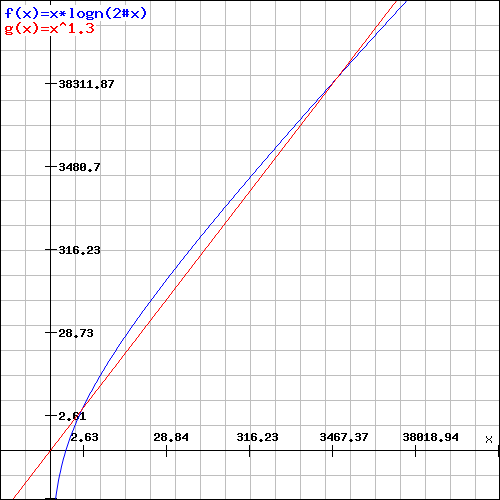
\includegraphics[
        width=10cm,
        keepaspectratio,
    ]{chapters/1. Anzahl der Vergleiche/img/lognplot.png}
    \caption{Ab $n=982$ wächst $n^{1.3}$ schneller als $n\ log\ n$.}
\label{fig:lognplot}
\end{figure}

Wegen $\Omega(n\ log\ n)$ interessieren wir uns für die Intervalle$\footnote{siehe dazu auch Tabelle~\ref{tab:calls}}:

\begin{itemize}
     \item $n\ log\ n \leq c4 \leq n^{1.3}$
     \item $n\ log\ n \leq n^{1.3} \leq c4 \leq n^2$
\end{itemize}

Die Ausführung des Tests zeigt, dass die Aufrufanzahl von $c4$ bei großen $n$ unterhalb $n^{1.3}$ oder zwischen $n^{1.3}$ und $n^2$ liegt:

\blockquote[{\cite[31]{She59}}]{
It appears that the time required to sort $n$ elements is proportional to $n^{1.226}$.\footnote{
\textit{Shell} führt in seinem Paper keinen Beweis auf. Er stützt seine Behauptung auf Messungen, die er selber in Tests durchgeführt hat: ``[...] an analytical determination of the expected speed has eluded the writer. However, experimental use has
established its speed characteristics.`` (ebenda)
}
}

\subsection*{Laufzeitanalyse}

Für die nachfolgenden Betrachtungen sei eine Eingabegröße $n = 2^p$ gegeben.
Die Inkremente $h$ entsprechen der über die Implementierung vorgegebenen Folge $h$ mit
$h_t = \frac{n}{2}, h_{t-1} = \frac{n}{4}, \dots, h_1 = 1$.
\\

Für die Analyse ist die \textbf{Shellsort}-Implementierung in Listing~\ref{lst:shellsort}) gegeben.

\begin{lstlisting}[language=java,label=lst:shellsort,caption={Implementierung des Shellsort-Algorithmus.}]

public static int[] sort(int[] arr) {

    int n = arr.length;
    int delta = n/2;
    int min;
    int j;

    while (delta > 0) { // c1

        for (int i = delta; i < arr.length; i++) {

            // c2

            min = arr[i];
            j = i;

            while (j - delta >= 0 && min < arr[j - delta]) {

                // c3;

                arr[j] = arr[j - delta];
                j -= delta;
            }
            arr[j] = min;
        }

        delta = delta / 2;

    }
    return arr;
}

\end{lstlisting}


Im Folgenden betrachten wir die Anzahl für die im Code durch Kommentare markierten Stellen $c1$ in Zeile 11, $c2$ in Zeile 13 und $c3$ in Zeile 20.

\\
Für eine erste \textit{worst-case}-Analyse ist ein Feld der Länge $16$ gegeben, in absteigender Reihenfolge sortiert (s. Abbildung~\ref{fig:bestcase})

\begin{figure}[h]
    \centering
    
\includegraphics[
        width=15cm,
        keepaspectratio,
    ]{chapters/1. Anzahl der Vergleiche/img/bestcase-sequence.png}
    \caption{Die für die Laufzeitabschätzung verwendete Eingabefolge $16..1$}
\label{fig:bestcase}
\end{figure}

\\

Ganz offensichtlich gilt für \textbf{c3}, dass es $lg(n)$-mal aufgerufen wird\footnote{hier wie im folgenden ohne Betrachtung der Schleifenbedingung, die an dieser Stelle insgesamt $lg(n) + 1$-mal aufgerufen wird}.
\\

\textbf{c2} befindet sich im Block der durch die in Zeile 11 definierten Zählschleife.

Der Startwert für \code{i} ist in jedem Durchgang des Blocks $c1$ der aktuelle Wert von \code{delta}\footnote{${8, 4, 2, 1}$ für das gegebene Beispiel}, und läuft jeweils bis $n - 1$.

In einem kompletten Durchlauf der Schleife enstpricht die Anzahl der Aufrufe von $c2$ also

\begin{equation}
(n - 1) - delta + 1 = n - delta
\end{equation}

\begin{tcolorbox}
    \textbf{Hinweis:}
    \\
    Für das Beispiel betrachten wir der Einfachheit halber Feldlängen der Form $2^p$.
    \\
    Für den allgemeinen Fall gilt für die Anzahl der Aufrufe von $c2$:\\

    \begin{equation}
        %\label{eq:dynamic_diag}
        \nonumber
        \sum_{i=1}^{\lfloor lg(n) \rfloor} n - \lfloor \frac{n}{2^i} \rfloor = n * lg(n) - \sum_{i=1}^{\lfloor lg(n) \rfloor} \lfloor \frac{n}{2^i} \rfloor
    \end{equation}
\end{tcolorbox}

Für die  Gesamtzahl der Aufrufe von $c2$ ergibt sich somit unter Berücksichtigung von $c1$

\begin{equation}
\sum_{i=1}^{lg(n)} n - \frac{n}{2^{i-1}}
\end{equation}

was nach Auflösen

\begin{equation}
    n * lg(n) - n + 1
\end{equation}

entspricht, und für unser Beispiel

\begin{equation}
    16 * lg(16) - 16 + 1 = 49
\end{equation}

ist.


\setlength{\tabcolsep}{0.8em}
{\renewcommand{\arraystretch}{1.7}%
\begin{table} %[hbtp]
    \begin{center}
        \begin{tabular}{|c |c |c |c | c| c| c}
            \hline
            \textbf{n} & \textbf{c2}  &  \textbf{$O(n^{1.1})$} & \textbf{$O(n^{1.3})$} & \textbf{$O(n\ log\ n)$} & \textbf{$O(n^2)$}  \\


            \hline
            $8$ & $17$  & \cellcolor{green!25}$9$ & \cellcolor{green!25}$14$ &  \cellcolor{red!25}$24$ & \cellcolor{red!25}$64$\\
            \hline
            $16$ & $49$ & \cellcolor{green!25}$21$ & \cellcolor{green!25}$36$ &\cellcolor{red!25}$64$ & \cellcolor{red!25}$256$ \\
            \hline
            $32$ & $129$ &  \cellcolor{green!25}$45$ & \cellcolor{green!25}$90$ & \cellcolor{red!25}$160$ &\cellcolor{red!25}$1024$ \\
            \hline
            $64$ & $321$ &  \cellcolor{green!25}$97$ & \cellcolor{green!25}$222$ & \cellcolor{red!25}$384$ & \cellcolor{red!25}$4096$ \\
            \hline
            $128$ & $769$ &   \cellcolor{green!25}$207$ & \cellcolor{green!25}$548$ & \cellcolor{red!25}$896$ & \cellcolor{red!25}$16.384$ \\

            \hline
            $256$ & $1793$ &   \cellcolor{green!25}$445$ & \cellcolor{green!25}$1351$ & \cellcolor{red!25}$2048$ & \cellcolor{red!25}$65.536$ \\
            \hline

            $1024$ & $9217$ &   \cellcolor{green!25}$2048$ & \cellcolor{green!25}$8192$ & \cellcolor{red!25}$10240$ & \cellcolor{red!25}$1.048.576$ \\
            \hline

            .. & & & & &  \\
            \hline
            $2156$ & $21.565$ &   \cellcolor{green!25}$4.645,29$ & \cellcolor{green!25}$21.564,69$ & \cellcolor{red!25}$23.875,84$ &\cellcolor{red!25}$4.648.336$ \\  \hline
            $2157$ & $21.576$ &  \cellcolor{green!25}$4.647,66$ & \cellcolor{red!25}$21.577,70$ & \cellcolor{red!25}$23.888,36$ &\cellcolor{red!25}$4.652.649$  \\  \hline
            $2158$ & $21.586$ &  \cellcolor{green!25}$4.650,03$ & \cellcolor{red!25}$21.590,70$ & \cellcolor{red!25}$23.900,88$ & \cellcolor{red!25}$4.656.964$  \\
            \hline
            ..  & & & & &  \\
            \hline
            $10.000$ & $120.005$ &    \cellcolor{green!25}$25118$ & \cellcolor{red!25}$158.489$ & \cellcolor{yellow!25}$132.877$ &\cellcolor{red!25}$1.0E8$ \\
            \hline

            $100000$ & $1.500.006$ &   \cellcolor{green!25}$316.227$ & \cellcolor{red!25}$3.162.277$ & \cellcolor{yellow!25}$1.660.964$ &  \cellcolor{red!25}$1.0E10$ \\
            \hline

            $200000$ & $3.200.006$ &   \cellcolor{green!25}$677.849$ & \cellcolor{red!25}$7.786.440$ & \cellcolor{yellow!25}$3.521.928$ &\cellcolor{red!25}$4.0E10$ \\
            \hline

            $500.000$ & $8.500.007$  &  \cellcolor{green!25}$1.857.235$ & \cellcolor{red!25}$2.56..E7$ & \cellcolor{yellow!25}$9.465.784$ & \cellcolor{red!25}$2.5E11$ \\
            \hline
            $1.000.000$ & $18.000.007$ & \cellcolor{green!25}$3.981.071$ & \cellcolor{red!25}$6.30..E7$ & \cellcolor{yellow!25}$1.99..E7$ & \cellcolor{red!25}$1.0E12$ \\
            \hline
        \end{tabular}
        \caption{Die Aufrufzahlen für $c2$ für verschiedene $n$. Schlüsselvergleiche spielen an dieser Stelle keine Rolle. Grün hinterlegte Werte sind kleiner als $c2$, rote sind größer. Mit $n > 2156$ wächst $O(n^\frac{4}{3})$ schneller als $c2$ und mit $n >= 982$ schneller als $O(n\ log\ n)$.
        }
        \label{tab:calls}
    \end{center}
\end{table}


In dem durch die in Zeile 18 definierte \code{while}-Schleife findet die eigentliche Arbeit des Algorithmus statt: Es wird überprüft, ob $delta$-entfernte Elemente in aufsteigender Reihenfolge sortiert angeordnet sind.

Ist das nicht der Fall, werden die Elemente an den Stellen $j$ und $j - delta$ ausgetauscht, bis die $h$-Folge sortiert ist.

Für den ersten Durchgang des Algorithmus an dieser Stelle mit $h_4 = 8$ ergibt sich somit die in Abbildung~\ref{fig:bestcase-it1} dargestellte Reihenfolge der Schlüssel:

\begin{figure}[h]
    \centering
    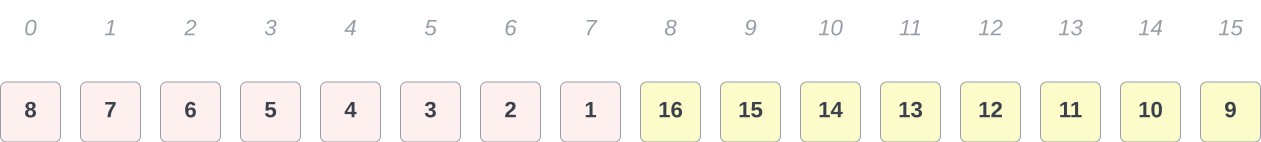
\includegraphics[
        width=15cm,
        keepaspectratio,
    ]{chapters/1. Anzahl der Vergleiche/img/bestcase-it1.png}
    \caption{Nach dem ersten Durchgang sind die Schlüssel in den Abständen $h_4 = 8$ sortiert, es ergeben sich zwei sortierte Teilfolgen der Länge $8$ }
    \label{fig:bestcase-it1}
\end{figure}

Die weiteren Durchgänge des Algorithmus sortieren das Feld entsprechend der Größe $h$: Es sind danach jeweils Schlüssel mit den Abständen $4$ (Abbildung~\ref{fig:bestcase-it2}), $2$  (Abbildung~\ref{fig:bestcase-it3}), und im letzten Schritt vollständig sortiert (Abbildung~\ref{fig:bestcase-it4}):

\begin{figure}[h]
    \centering
    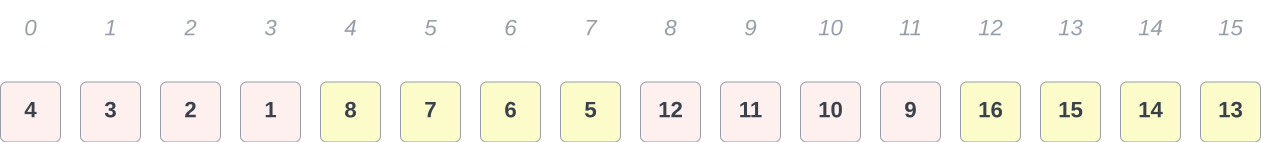
\includegraphics[
        width=15cm,
        keepaspectratio,
    ]{chapters/1. Anzahl der Vergleiche/img/bestcase-it2.png}
    \caption{Die Sortierung für $h_3 = 4$, es sind 4 Folgen, deren Schlüssel jeweils den Abstand $4$ haben. }
    \label{fig:bestcase-it2}
\end{figure}

\begin{figure}[h]
    \centering
    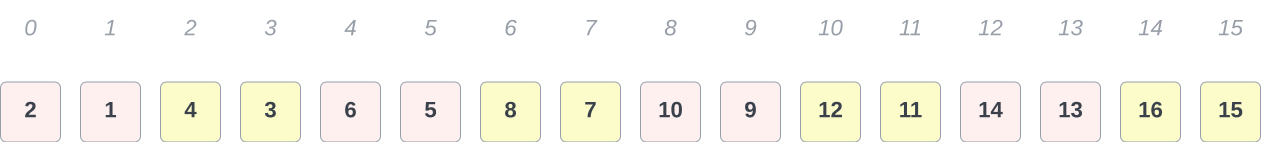
\includegraphics[
        width=15cm,
        keepaspectratio,
    ]{chapters/1. Anzahl der Vergleiche/img/bestcase-it3.png}
    \caption{Im vorletzten Sortierschritt sind $8$ Folgen der Länge $2$ sortiert. }
    \label{fig:bestcase-it3}
\end{figure}

\begin{figure}[h]
    \centering
    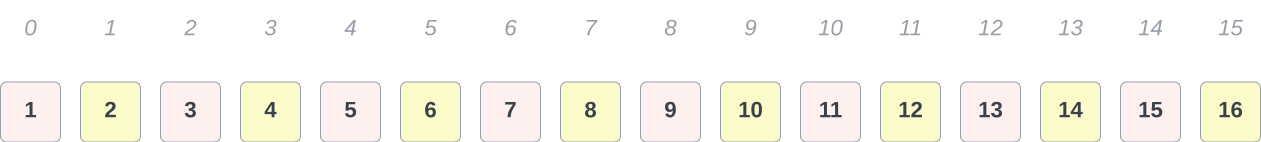
\includegraphics[
        width=15cm,
        keepaspectratio,
    ]{chapters/1. Anzahl der Vergleiche/img/bestcase-it4.png}
    \caption{Der letzte Durchgang des Algorithmus vergleicht Schlüssel mit Distanzfolgen der Länge $1$, also direkt benachbarte Schlüssel. }
    \label{fig:bestcase-it4}
\end{figure}

\\
Für die Berechnung der Anzahl der Aufrufe von $c3$ stellt man fest, das in diesem Fall in jedem Schritt \textit{immer} 2 Elemente, die eine Distanz von $h_s$ aufweisen, falsch sortiert sind.

Der Algorithmus tauscht also in diesem Fall in jedem Durchgang alle Schlüssel untereinander aus, die er über \code{min < arr[j-delta]} miteinander vergleicht, was folglich die maximale Anzahl von Schlüsselvertauschungen in dieser vergleichsbasierten Implementierung für ein Feld der Größe $n$ ergibt, nämlich $\frac{n}{2}$.
Insgesamt finden dadurch für $c3$

\begin{equation}
    lg(n) * \frac{n}{2}
\end{equation}

Aufrufe statt.

Mit der Anzahl der berechneten Aufrufe $c1, c2, c3$ ergibt sich somit für die Laufzeit $T(n)$ für diesen Fall


\begin{equation}
    lg(n) + n * lg(n) - n + 1 +  lg(n) * \frac{n}{2}
\end{equation}

und zusammengefasst

\begin{equation}\label{eq:bestcase}
 f(n) = \frac{3}{2} * n * lg(n) + lg(n) - n + 1
\end{equation}

was nach Einsetzen zu

\begin{equation}
    lg(16) + 16 * lg(16) - 16 + 1 +  lg(16) * \frac{16}{2} = 85
\end{equation}

Aufrufen für unser Beispiel  führt.
\\

\subsection*{Nachweis der Komplexitätsklasse}
Um $O$ zu ermitteln, werden nun alle Konstanten der Funktion~\ref{eq:bestcase} eliminiert, und der ``dominante`` Summand in Abhängigkeit von $n$ betrachtet, der in diesem Fall $lg(n) * n$ ist.

Wir vermuten ein $N-log-N$-Wachstum\footnote{
    mit $O(log\ n)$ bzw $O(n\ log\ n)$ nehmen wir für die $O$-Notation wieder die in der Fachliteratur gebräuchlichere Schreibweise auf. Sowohl \textit{Güting und Dieker} als auch \textit{Ottmann und Widmayer} weisen in \cite[15]{GD18a} bzw. \cite[5]{OW17a} darauf hin, dass die Angabe der Basis keine Rolle spielt, da sich Logarithmen mit verschiedenen Basen ohnehin nur durch einen konstanten Faktor unterscheiden (es gilt $log_a(x) = \frac{log_b(x)}{log_b(a)}$).
} (vgl.~\cite[5]{OW17a}), und wollen nun zeigen, dass $T(n)$ in $O(n\ log\ n)$ liegt.
\\
Hierfür müssen wir ein geeignetes $c$ und ein $n_0$ finden, so dass gilt:

\begin{equation}
    f \in O(n\ log\ n): \leftrightarrow \exists n_0 \in \mathbb{N}, c \in \mathbb{R}, c > 0: \forall n \geq n_0: f(n) \leq c * n*lg(n)
\end{equation}

(vgl. \cite[11]{GD18a}).

\begin{proof}\label{pr:nlogn}
    \\
Zu zeigen ist
\begin{equation}
\frac{3}{2} * n * lg(n) + lg(n) - n + 1 \leq c * n * lg(n)
\end{equation}

Wir wählen für $n_0 = 1$  und $c = \frac{3}{2}$, denn es gilt sicher $\forall n \geq n_0: \frac{3}{2} * n * lg(n)  \leq \frac{3}{2} * n * lg(n)$.

Ausserdem gilt stets $\forall n \in \mathbb{N}: lg(n) < n$, woraus $lg(n) - n < 0$ folgt, und damit auch $lg(n) - n + 1 \leq 0$.
\\
Insgesamt gilt also

\begin{equation}
n_0 = 1, c = \frac{3}{2}: \forall n \geq n_0: \frac{3}{2} * n * lg(n) + lg(n) - n + 1 \leq c * n * lg(n)
\end{equation}

    womit $f = O(n * log(n))$ gezeigt ist.\square
\end{proof}

\subsection*{Worst-Case-Analyse}

Unter der Annahme, dass ein in umgekehrter Reihenfolge sortiertes Feld zu einer Laufzeit von $O(n^2)$ bei dem \textbf{Shellsort}-Algorithmus führt, konnten wir mit dem in dem vorherigen Abschnitt gewählten Parametern nur eine Laufzeit von $O(n\ log\ n)$ nachweisen.
\\

Tatsächlich stellt der Anwendungsfall nicht den worst-case für den Algorithmus dar, da ja gerade diese Form von Sortierreihenfolge dem Algorithmus die Vorsortierung der $h$-Folgen ermöglicht:
\\
\blockquote[{\cite[3]{Pra72}}]{
    The idea underlying Shellsort is that moving elements of A long
    distances at each swap in the early stages, then shorter distances later,
    may reduce this $O(n^2)$ bound.
}
\\

Es gilt also, die Vorsortierung auszuhebeln.
\\

Für \textbf{Insertion-Sort} ist die Laufzeit im worst-case $O(n^2)$ (vgl.~\cite[87]{OW17b}). Da Shellsort mindestens im letzten Schritt diese Sortiermethoden auf Distanzfolgen der Länge $1$ anwendet, muss der Algorithmus eine Folge als Eingabe erhalten, die durch die ersten $lg(n) - 1$-Durchgänge (mit $h_s = 2^{s - 1}, 1 <= s < lg(n)$) \underline{keine} Änderungen an der Schlüsselfolge vornimmt, um dann im allerletzten Schritt \underline{alle} Daten zu sortieren, was maximal $\frac{n}{2}$ Inversionen bedeutet zuzüglich der benötigten Verschiebe-Operationen.
\\
Hierzu kann wie im vorherigen Beispiel für $n=16$ ein Feld mit folgender Schlüsselanordnung verwendet werden: Felder mit geradem Index enthalten kleinere Schlüssel als Felder mit ungeradem Index.
Hier gilt für alle Elemente aus dem Feld $A$:

\begin{equation}
\forall i, j \in \mathbb{N}_{[0, n - 1]}, 2 \mid i, 2 \nmid j:  A[i] < A[j] \land A[i] < A[i + 1] \land A[j] < A[j +1]
\end{equation}

Abbildung~\ref{fig:worstcase-sequence} veranschaulicht die Anordnung.

\begin{figure}[h]
    \centering
    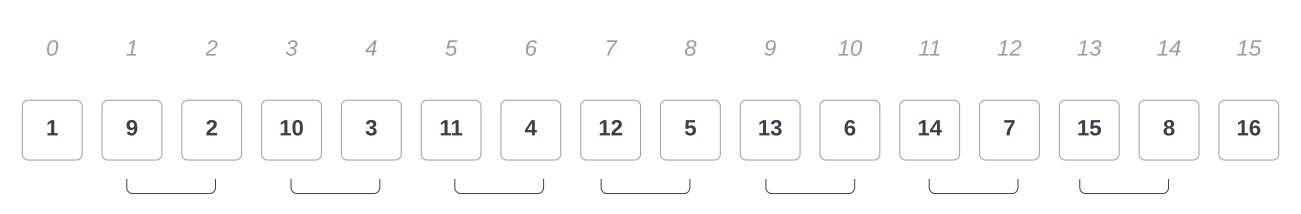
\includegraphics[
        width=15cm,
        keepaspectratio,
    ]{chapters/1. Anzahl der Vergleiche/img/worstcase-sequence}
    \caption{Eine \textit{worst-case} Schlüsselfolge für Shellsort. Felder mit geradem Index enthalten kleinere Schlüssel als Felder mit ungeradem Index.}
    \label{fig:worstcase-sequence}
\end{figure}

Markiert sind die direkt benachbarten Felder, die eine \textit{Inversion} aufweisen\footnote{
in diesem Zusammenhang bedeutet Inversion: \textit{Fehlstellung} (vgl.~\cite[87]{OW17b})
}, die im letzten Schritt des Algorithmus eine bzw. mehrere Verschiebungen bedingen.
\\
In den vorherigen Schritten - also bei den Durchgängen mit Distanzfolgen $h_s > 1$, findet der Algorithmus jeweils Schlüssel in korrekter Sortierreihenfolge vor.


Mit $h_4 = 8$ werden die Felder $A[0..7]$ mit den Feldern $A[8..15]$ verglichen - hier gilt in jedem Fall, dass die Schlüssel $A[i] < A[j] (\forall i < j, j - i = 8)$ sind.

Auch im darauffolgenden Durchgang ($h_3 = 4, j - i = 4$) finden keine Verschiebungen statt, da keine Inversion gefunden wird.
Erst im letzten Schritt, in dem direkt benachbarte Elemente miteinander verglichen werden, werden die Inversionen ermittelt und die Verschiebung der Elemente findet statt (s. Abbildung~\ref{fig:worstcase-sortsequence}).

\begin{figure}[h]
    \centering
    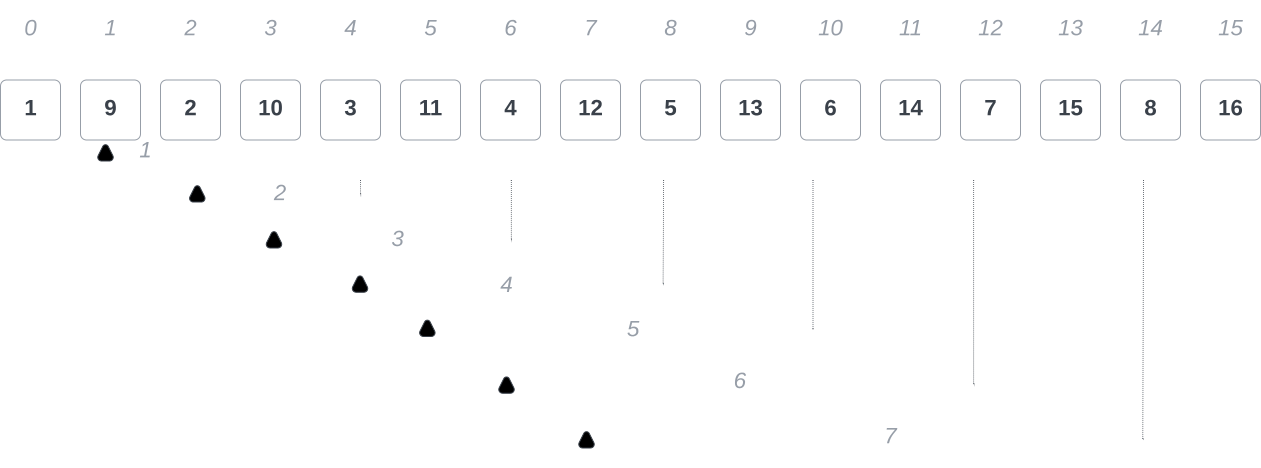
\includegraphics[
        width=15cm,
        keepaspectratio,
    ]{chapters/1. Anzahl der Vergleiche/img/worstcase-sortsequence}
    \caption{Für die \textit{worst-case} Schlüsselfolge werden im letzten Schritt 7 Fehlstellungen festgestellt. Jede Fehlstellung bedingt eine Verschiebung um die angegebene Anzahl von Positionen.}
    \label{fig:worstcase-sortsequence}
\end{figure}

In diesem Fall wird $c3$ insgesamt $32$ mal aufgerufen.
\\
Da jeweils zwei Schlüssel bereits korrekt sortiert sind ($A[0]$ und $A[n-1]$) existieren noch $\frac{n}{2} - 1$ Inversionen.
Jede Inversion erzwingt eine Verschiebung des größten Elements um $\frac{i}{2}$ Positionen nach links.
\\
Für die Berechnung der Laufzeitkomplexität ergibt sich somit der Term

\begin{equation}
    \sum_{i=1}^{\frac{n}{2} - 1} i = \frac{\frac{n}{2}(\frac{n}{2} - 1)}{2} = \frac{n^2 - 2n}{8}
\end{equation}

und unter Berücksichtigung der Terme für $c1$, $c2$, $c3$ die Funktion

\begin{equation}
    f(n) = lg(n) + n * lg(n) - n + 1 +  \frac{n^2 - 2n}{8}
\end{equation}

was zu einer Laufzeitabschätzung von $O(n^2)$ führt.